\documentclass{article}

\usepackage{graphicx}
\usepackage{amsmath}
\usepackage{siunitx}

\title{Mapping circuit to transfer function}
\author{Anderson Hsieh}
\date{August 5, 2026}

\begin{document}

\maketitle

\section{Questions Answered}
    \subsection{solving RC circuit : rc1}
    so we have a RC circuit, we find its transfer function 
    \begin{align*}
        H(s)&=\frac{V_{out}(s)}{V_{in}(s)}\\
        V_{out}(s)&=V_{in}(s)*\frac{Z_c}{Z_c+Z_R}\\
        V_{out}(s)&=V_{in}(s)*\frac{\frac{1}{sC}}{\frac{1}{sC}+R}\\
        H(s)&=\frac{\frac{1}{sC}}{\frac{1}{sC}+R}\\
    \end{align*}
    $V_{in}(s) = 1$ because input is a AC source with amplitude of 1\\
    say 
    \begin{align*}
        C = \SI{1}{\pico\farad} = \SI{1e-12}{\farad}, R = \SI{1}{\kilo\ohm} = \SI{1e3}{\ohm}\\
    \end{align*}
    
    for a purely resistive load, we have the following relationship for power vs voltage
    \begin{align*}
        P_{\text{load}}&= V_{\text{out,rms}}
         \left(\frac{V_{\text{out,rms}}}{R_{\text{load}}}\right) \\
         &= \frac{V_{\text{out,rms}}^2}{R_{\text{load}}}.
    \end{align*}

    at -3dB cut off frequency, power delivered to a load with resistance R drops to half.
    \begin{align*}
        \frac{P_{\mathrm{current}}}{P_{\mathrm{max}}}&= \frac{1}{2} \\
        \left(\frac{V_{\mathrm{current}}}{V_{\mathrm{max}}}\right)^2&= \frac{1}{2} \\
        \frac{V_{\mathrm{current}}}{V_{\mathrm{max}}}&= \sqrt{\frac{1}{2}} \\
            &= \frac{1}{\sqrt{2}} \\
            &\approx 0.7071
    \end{align*}


    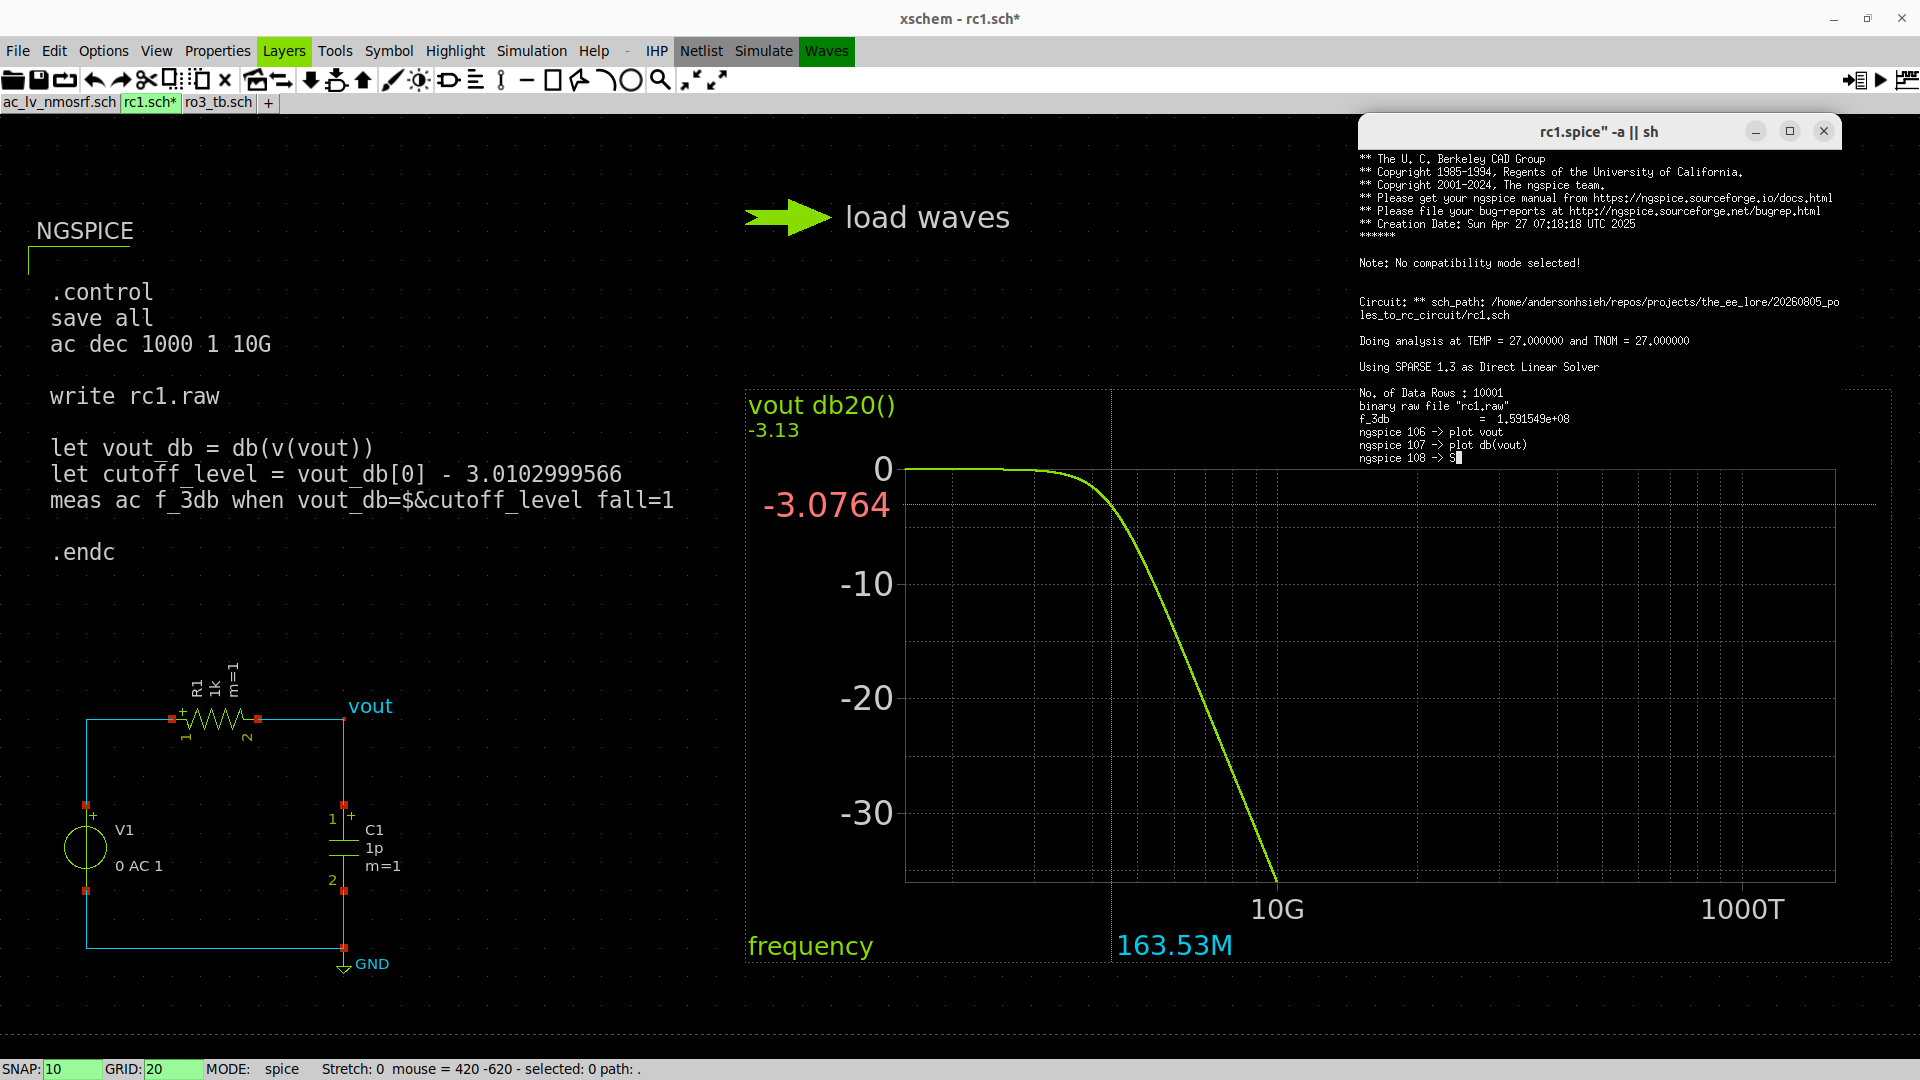
\includegraphics[width=\textwidth]{images/rc1.png}
\section{Questions To Be Answered}
    \begin{enumerate}
        \item how do they tune VDD for ring oscillator in a real application?
        \item poles and zeros in oscillators
        \item current mirrors in differential ring oscillator
    \end{enumerate}
\section{Some Picture}
\end{document}
